\subsection{Summary of the results} \label{subsec:Summary}

In this section we summarize all the above results into Table~\ref{table:compareTable} and Fig.~\ref{fig:LWEPlots}. To make the overview complete, we include the results on asymptotic analysis of \BKW algorithm \cite{DCC:ACFFP15, C:KirFou15, DCC:HKM} and the linearization attack by Arora-Ge \cite{ICALP:AroGe11}.

The most important part of the table is the middle-column showing the constants in the exponents of the algorithms' runtimes. These constants are functions of \LWE parameters $\cq, \ca = \TLandau(1)$ and the constant $\cBKZ$ -- the exponent of the running time of \SVP solver called within \BKZ.

The upper part of the table states the complexities of attacks when only $\poly(n)$ memory is available. Only lattice-based attacks are applicable in this setting. In this part of the table, running times of all the algorithms are of order $2^{\TLandau(n \log n)}$. The reader should not be confused with the exponential number of samples and polynomial memory for the \DUAL attack: as explained in Sect.~\ref{sec:OtherAttacks}, we do not have to store all the samples at once. Since for Kannan's enumeration we have the term  $\smash{\sqrt{2 \cBKZ} = \sqrt{1/e} \approx 0.42}$ in the denominator, \BKZ+\ENUM is faster than \DUAL or \Embed algorithms when the number of samples is limited. The \DUAL attack, however, is asymptotically faster with $2^{\TLandau(n)}$ samples: the additive term $\sfrac12$ is slightly larger than $0.42$.

In the lower part of the table, exponential space-complexity is allowed resulting in single-exponential running times for the attacks. In this case, \emph{all} lattice-based attacks ($\BKZ+\ENUM$, \DUAL, \Embed) have the \emph{same} constants provided we can access only $\poly(n)$ \LWE samples. Exponential memory complexity comes from the lattice-basis reduction. The \DUAL attack, unlike other \emph{lattice-based} algorithms, can profit from exponential number of samples: the constant gets improved by the additive term of $\sfrac12$. Since the \DUAL attack needs exponentially many samples, this $\sfrac12$ term vanishes when we have a limited number of samples, in which case we have to run the amplification process. Recall that as the result of the amplification, a `fresh' \LWE sample of the form $(\avec', t')$ is produced, where $(\avec' = \AMat \xvec \bmod q, t' = \ScProd{\tvec}{\xvec} \bmod q)$ for some constant-width Gaussian $\xvec \in \Z_q^m$. It is easy to verify that in case of $\TLandau(n\log n)$ samples, the noise-rate in $t'$ increases exactly by $\sfrac12$, thus making the whole attack slightly worse. 

In case the number of samples is only linear in $n$, i.e. $m = \cm n$ for some constant $\cm$, the amplification works only for certain range of parameters $\cm, \cq, \ca$. This is due to the fact that we amplify the samples with a Gaussian $\xvec$ of a \emph{non-constant} width of order $\TLandau(n^{a})$ for some $a=\TLandau(1)$. In case $\ca<1/2+\cq/\cm$, or in other words, the noise in the original samples is too large relative to the modulus $q$, the standard deviation of the amplified samples will become larger than $q$. We refer the reader to \cite[Lemma 10]{DCC:HKM} for the details.

The same situation happens for the combinatorial \BKW algorithms, since we can again use amplification to produce enough samples for the algorithm to work. As opposed to the \DUAL attack, \BKW works only with exponential memory at disposal as it has to store many samples at once. 
Further, note that the denominators of the exponents for lattice-based attacks and for \BKW are the same except they are squared for the former. As a consequence, as soon as $\ca$ (or $\ca+\sfrac12$ for $2^{\TLandau(n)}$ many samples) is greater than 1, lattice-based techniques will outperform \BKW. Essentially it means that lattice-based attacks are better for low-noise rates.

Yet this is not always the case if we compare lattice-based attacks with the recent improvement for the \BKW algorithm by Kirchner-Fouque \cite{C:KirFou15} and Guo et al.\ \cite{C:GuoJohSta15}, which we name $\BKW2$. Its constant $\bigl(\sfrac{1}{\cq} + 2\ln(\tfrac{\cq}{\cq-\ca})\bigr)$ (in case of $2^{\TLandau(n)}$ many samples) is always smaller than the constant $\frac{\cq}{\ca+1/2}$ of \BKW, but not necessarily smaller than the constant for the lattice-based attacks. It hugely depends on the value $\cBKZ$ that obviously impacts their complexity. How exactly these all constants compare with each other is illustrated in Fig.~\ref{fig:LWEPlots}.

  
In the upper figure we compare single-exponential attacks with \emph{polynomial} number of \LWE samples. If we order the algorithms relative to the value of their constant for the parameters $(\cq, \ca)$, differently coloured areas correspond to different orderings. Since the constants for lattice-based attacks heavily rely on the value $\cBKZ$, we distinguish the two cases: (1) $\cBKZ = 1$ (Aggarwal et al. \cite{STOC:ADRS15} provable instantiation of an \SVP solver), and (2) $\cBKZ = 0.292$ (heuristic \SVP algorithm from \cite{SODA:BDGL16}). The subscript in the name of lattice-based attack indicates which case is chosen.  

For example, the orange area marks the range of \LWE parameters $(\cq, \ca)$ where the $\BKZ+\ENUM$ attack with $\cBKZ = 0.292$ performs better than $\BKW2$. For small values of $\ca$, however, \BKW algorithms outperform lattice-based techniques. This is due to the fact that combinatorial attacks are more robust to large-noise instances (the smaller $\ca$, the larger Gaussian width $\alpha q = n^{\cq - \ca}$), while lattice-based algorithms seem to perform significantly worse for an increased error-rate. We note that in case of $\poly(n)$ samples, by \ENUM we mean all the lattice-based attacks as they have the same constant.

We present the same figure for the case of \emph{exponential} number of samples. Here we take only the \DUAL algorithm to compare with \BKW. Notice that the horizontal areas (blue at the top and pink at the bottom) get shifted by $1/2$ comparatively to the upper figure -- the gain we have in the exponents for $\BKW$ and $\DUAL$ algorithms once we have exponentially many samples.

In both figures, the area below the green line denotes the values of $\cq, \ca$ for which hardness reductions (both classical and quantum) hold. As an example, for parameters $(\cq=2, \ca = 0.5)$ -- the values chosen for the cryptosystem described in \cite{STOC:Regev05} -- we make the constants explicit. 

%
% Table
%

\renewcommand{\arraystretch}{1.7}
\begin{table}[h]
	\begin{center}
		\begin{tabular}{|p{6.3cm} |c | c |}   \hline
			\multicolumn{3}{|c|}{$\rho(\ALG) = \frac{T(\ALG)}{\Psucc(\ALG)},$ \; $M=\text{Space}$} \\ \thickline 
			\multirow{2}{5.49cm}{\centering \textbf{polynomial memory}}& \multicolumn{2}{c|}{\cellcolor{gray!10}{$M=\poly(n), T(\BKZ) = 2^{\cBKZ n \log n}$}} \\ \cline{2-3} 
			& $\log(\rho) / (n \log n)$ & \# Samples \\ \hline
			\multicolumn{3}{|c|}{\textsc{ Lattice-based algorithms}}\\ \hline
			$\BKZ+\ENUM$, where $\ENUM$ is: & \multirow{4}{*}{\raisebox{4.5ex}{$ \frac{2 \cBKZ \cdot \cq}{(\sqrt{2 \cBKZ}+\ca)^2}$}} &
			\multirow{4}{*}{\raisebox{4.5ex}{$\Theta(n)$}}  \\[-1.5ex] 
			-- Babai~(Sect.~\ref{sec:BabaisNP}) & &   \\[-1.5ex]
			-- Lindner-Peikert~(Sect.~\ref{sec:LPNP}) & & \\ [-1.5ex]
			-- \GenPrun~(Sect.~\ref{sec:GenPrun}) & & \\ \hline 
			\multirow{2}{*}{{$\Dual$ (Sect.~\ref{sec:OtherAttacks}, Thm.~\ref{thm:DualSearch})}} & $\frac{2 \cBKZ \cdot \cq}{ \vphantom{\scalebox{1.2}x^2} \ca ^2}  $  & $\Theta (n \log n)$ \\ \cline{2-3}
			& $\frac{2 \cBKZ \cdot \cq}{ ( \ca +1/2)^2 } $ &  $2^{\Theta(n)}$ \\ \hline
			Embedding~(Sect.~\ref{sec:OtherAttacks}, Thm.~\ref{thm:Embed}) &  $ \frac{2 \cBKZ \cdot \cq}{\vphantom{\scalebox{1.2}x^2} \ca^2} $ & $\Theta(n)$ \\[2pt] \thickline %\thicklines
			\multirow{2}{5.49cm}{\centering \textbf{exponential memory}}& \multicolumn{2}{c|}{\cellcolor{gray!10}{$M=2^{\Theta(n)}, T(\BKZ) = 2^{\cBKZ n}$}} \\ \cline{2-3}
			& $\log(\rho) / n$ & \# Samples \\ \hline
			%\multicolumn{3}{|c|}{\textsc{ Lattice-based algorithms}}\\ \hline
			$\BKZ+\ENUM$, where $\ENUM$ is: & \multirow{4}{*}{\raisebox{4.5ex}{$\frac{2 \cBKZ \cdot \cq}{\ca^2}$}} & \multirow{4}{*}{\raisebox{4.5ex}{$\Theta(n)$}}  \\[-1.5ex]
			-- Babai~(Sect.~\ref{sec:BabaisNP}) & &   \\ [-1.5ex]
			-- Lindner-Peikert~(Sect.~\ref{sec:LPNP}) & & \\ [-1.5ex]
			-- \GenPrun~(Sect.~\ref{sec:GenPrun}) & & \\ \hline 
			\multirow{3}{*}{$\Dual$ (Sect.~\ref{sec:OtherAttacks}, Thm.~\ref{thm:DualSearch}), \cite{DCC:HKM}} & $\frac{2 \cBKZ \cdot \cq}{ (\ca +1/2)^2 } $ &  $2^{\Theta(n)}$  \\[1pt] \cline{2-3}
			& $\frac{2 \cBKZ \cdot \cq}{\vphantom{\scalebox{1.2}x^2} \ca^2}  $  & $\Theta (n \log n)$ \\ \cline{2-3}
			& $\frac{2 \cBKZ \cdot \cq}{\vphantom{\scalebox{1.2}x^2} (\ca-\cq/\cm)^2}  $  & $(\cm+\smallo(1))n$ \\ \hline
			Embedding~(Sect.~\ref{sec:OtherAttacks}, Thm.~\ref{thm:Embed}) &  $ \frac{2 \cBKZ \cdot \cq}{\vphantom{\scalebox{1.2}x^2} \ca^2} $ & $\Theta(n)$ \\[2pt] \hline
			\multicolumn{3}{|c|}{\textsc{ Combinatorial algorithms}}\\ \hline
			\BKW  (\cite{DCC:ACFFP15}) & $\frac{1}{2} \frac{\cq}{\ca+1/2} $ & $2^{\Theta(n)}$ \\ \hline
			\multirow{2}{*}{\BKW (Thm.\ 8 in \cite{DCC:HKM})} & $\frac{1}{2} \frac{\cq}{ \ca} $ & $\Theta(n \log n)$ \\ \cline{2-3}
			& $\frac{1}{2} \frac{\cq}{ \ca-\cq/\cm} $ & $(\cm+\smallo(1)) n$ \\ \hline	
			\BKWKF (\cite{C:GuoJohSta15, C:KirFou15}) & $ \bigl(\sfrac{1}{\cq} + 2\ln(\tfrac{\cq}{\cq-\ca})\bigr)^{\scriptscriptstyle -1} $ & $2^{\Theta(n)}$ \\ \hline
			\multirow{2}{*}{\BKWKF (Thm.\ 8 in \cite{DCC:HKM})} & $ \bigl(2\ln(\tfrac{\cq}{\cq-\ca})\bigr)^{\scriptscriptstyle -1} $ & ${\Theta(n\log n)}$ \\ \cline{2-3}
			& $ \bigl(2\ln(\tfrac{\cq-\cq/(\cm-1)}{\cq-\ca})\bigr)^{\scriptscriptstyle -1} $ & $(\cm+\smallo(1)) n$ \\
			 \thickline
			Arora-Ge (\cite{APS15, ICALP:AroGe11}), $\cq-\ca < \sfrac12$ & \scriptsize{$ \omega \cdot (1-2\ca) \cdot  n^{2 \ca} \log^2(n)$} & $\bigO(2^{n^{\ca} \log^2 n})$ \\ \hline
			Arora-Ge (\cite{APS15, ICALP:AroGe11}), $\cq-\ca \geq \sfrac12$ & \scriptsize{$\omega \cdot (2 \ca-1) \cdot n \log(n)$} & $\bigO(2^{n \log n})$ \\ \hline
		\end{tabular} 
	\end{center}
	\caption[\LWE attacks: asymptotics]{Asymptotic comparison of algorithms for \LWE. We denote $q = \bigO(n^{\cq})$, $\alpha =  \bigO(1/n^{\ca})$ and $\cBKZ$ is the constant hidden in the run-time exponent of lattice-basis reduction. 
	In order to run the \BKW (resp. \BKW2) algorithm when only \emph{linear} number of samples is available, the \LWE parameters must satisfy $\ca>1/2+\cq/\cm $ (resp.\  $\ca>1/2+\cq/(\cm-1)$) and $\cq>\cq/\cm - 1/2$ (resp.\ $\cq>\cq/(\cm-1) - 1/2$).  Such constraints come from the amplification.
	For Arora-Ge, $2\leq \omega <3 $ is the linear algebra constant.}
	\label{table:compareTable}
\end{table}

%
% Figures
%

\definecolor{LightSkyBlue}{RGB}{135, 206, 250}
\definecolor{Orange}{RGB}{255, 165,0}
\definecolor{LightSalmon}{RGB}{255, 160, 122}
\definecolor{LeafGreen}{RGB}{34, 139,  34}


\begin{figure}[h]
		\begin{subfigure}[h]{0.99\textwidth}
		\centering
		\begin{tikzpicture}
				    \node[anchor=south west,inner sep=0] (image) at (0,0) {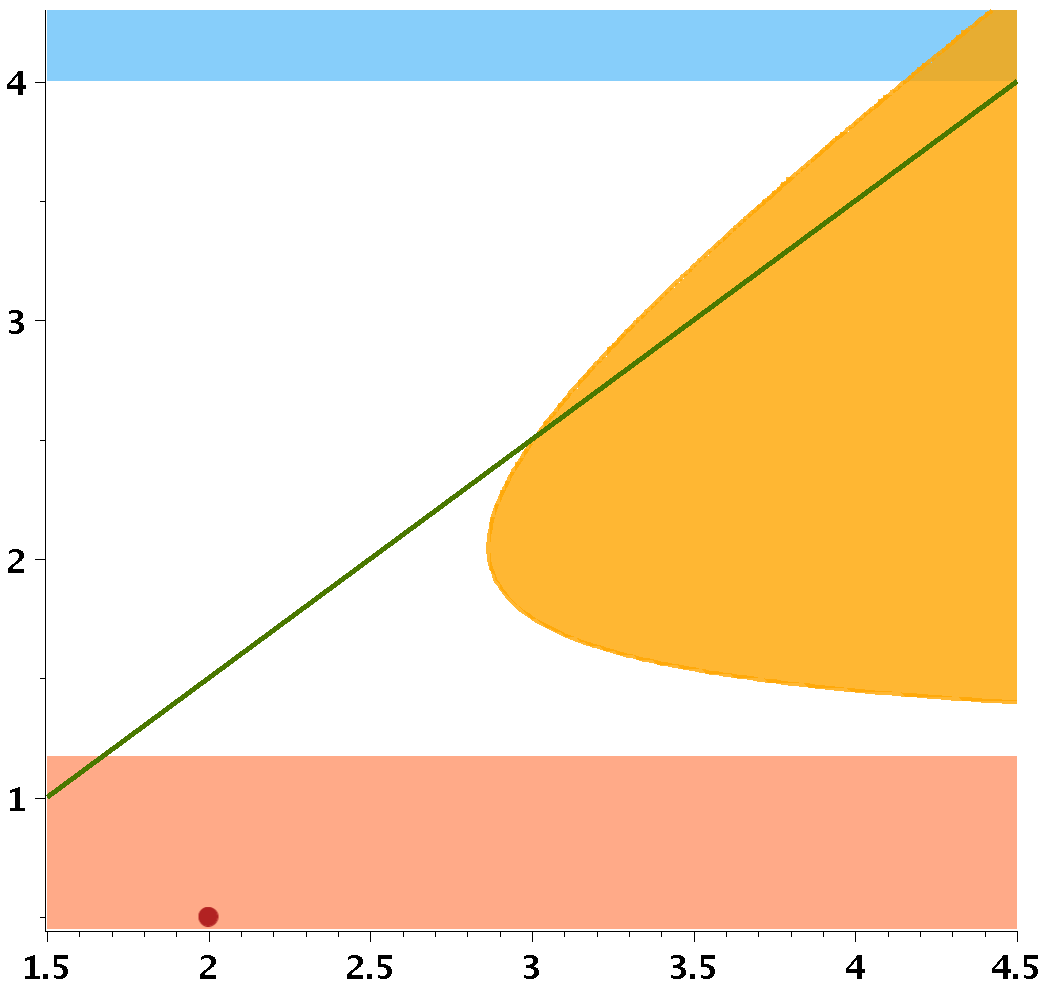
\includegraphics[width=0.60\textwidth]{Plots/Plots_SingleExp_PolySamples.png}};
				    \begin{scope}[x={(image.south east)},y={(image.north west)}]
				    	
				    	% Help lines: Comment out once finished % 
				   		%\draw[help lines,xstep=.1,ystep=.1] (0,0) grid (1,1);
				    	%\foreach \x in {0,1,...,9} { \node [anchor=north] at (\x/10,0) {0.\x}; }
				    	%\foreach \y in {0,1,...,9} { \node [anchor=east] at (0,\y/10) {0.\y}; }
				    	
				    	%\node[draw=none] at (0.45, 0.15) {\tiny $\BKW2 \leq \ENUM2 \leq \BKW \leq \ENUM$};
				    	%\node[draw=none, color=black] at (0.6, 0.52) {Quantum reduction};
				    
				    	\draw[fill=LightSkyBlue, opacity=0.9] (1.0, 0.6) rectangle (1.05, 0.65) node[yshift=-2ex, xshift=17ex]{$\ENUMH \leq \BKW2 \leq \ENUMOne \leq \BKW$};
				    	\draw[fill=Orange] (1.0, 0.5) rectangle (1.05, 0.55) node[yshift=-2ex, xshift=17ex] { $\ENUMH \leq \BKW2 \leq \BKW \leq \ENUMOne$}; 
				    	\draw[fill=LightSalmon, opacity=0.8] (1.0, 0.4) rectangle (1.05, 0.45) node[yshift=-2ex, xshift=17ex] {$\BKW2 \leq \BKW \leq \ENUMH \leq \ENUMOne $};
				    	\draw[fill=white] (1.0, 0.3) rectangle (1.05, 0.35) node[yshift=-2ex, xshift=17ex] {$\BKW2 \leq \ENUMH \leq \BKW \leq \ENUMOne$};
				    	
				    	\node[draw=none, xshift=14.5ex, yshift=1.5ex] at (0.05, 0.15) {\scriptsize $\BKW2 = 1.73$};
				    	\node[draw=none, xshift=13.5ex, yshift=1.5ex] at (0.05, 0.12) {\scriptsize $\BKW = 2.0$};
				    	\node[draw=none, xshift=16.5ex, yshift=1.5ex] at (0.04, 0.09) {\scriptsize $\ENUMH = 4.67$};
				    	\node[draw=none, xshift=15ex, yshift=1.5ex] at (0.05, 0.06) {\scriptsize $\ENUMOne = 16.0$};
				    	
				    	\node[draw=none, rotate=35] at (0.37, 0.42){$\alpha q > \sqrt{n}$};
				    	
				    	\node[draw=none] at (0.5, -0.03) {$\cq$};
				    	\node[draw=none] at (-0.02, 0.5) {$\ca$};
				    	
				    \end{scope}
		\end{tikzpicture}
		\caption[Comparison of algorithms for \LWE with polynomial number of samples]{
				 Comparison of \emph{single}-exponential attacks with \emph{polynomial} number of samples relative to the $(\cq, \ca)$ parameters. The orange area illustrates the parameter-ranges where a \BKZ-reduction instantiated with heuristic $\SVP$-solver (i.e.\ $\cBKZ=0.292$) followed by an enumeration algorithm $\ENUM$ beats the $\BKW2$ algorithm from \cite{C:GuoJohSta15, C:KirFou15}. For large values of $\ca$ depicted blue (i.e. small noise-rate), the enumeration algorithms are better than the combinatorial \BKW. On the other hand, \BKW performs better for higher-noise rates (pink area). The red dot denotes \LWE parameters considered in \cite{STOC:Regev05}: $\cq=2, \ca=0.5$. The area below the green line corresponds to the parameters $(\cq, \ca)$ for which the hardness reductions hold.
		}
		\label{fig:SingExpPolySamples}
		\end{subfigure} 
		
		\begin{subfigure}[h]{0.99\textwidth}
		\centering
		\vspace*{20pt}
		\begin{tikzpicture}
				    \node[anchor=south west,inner sep=0] (image) at (0,0) {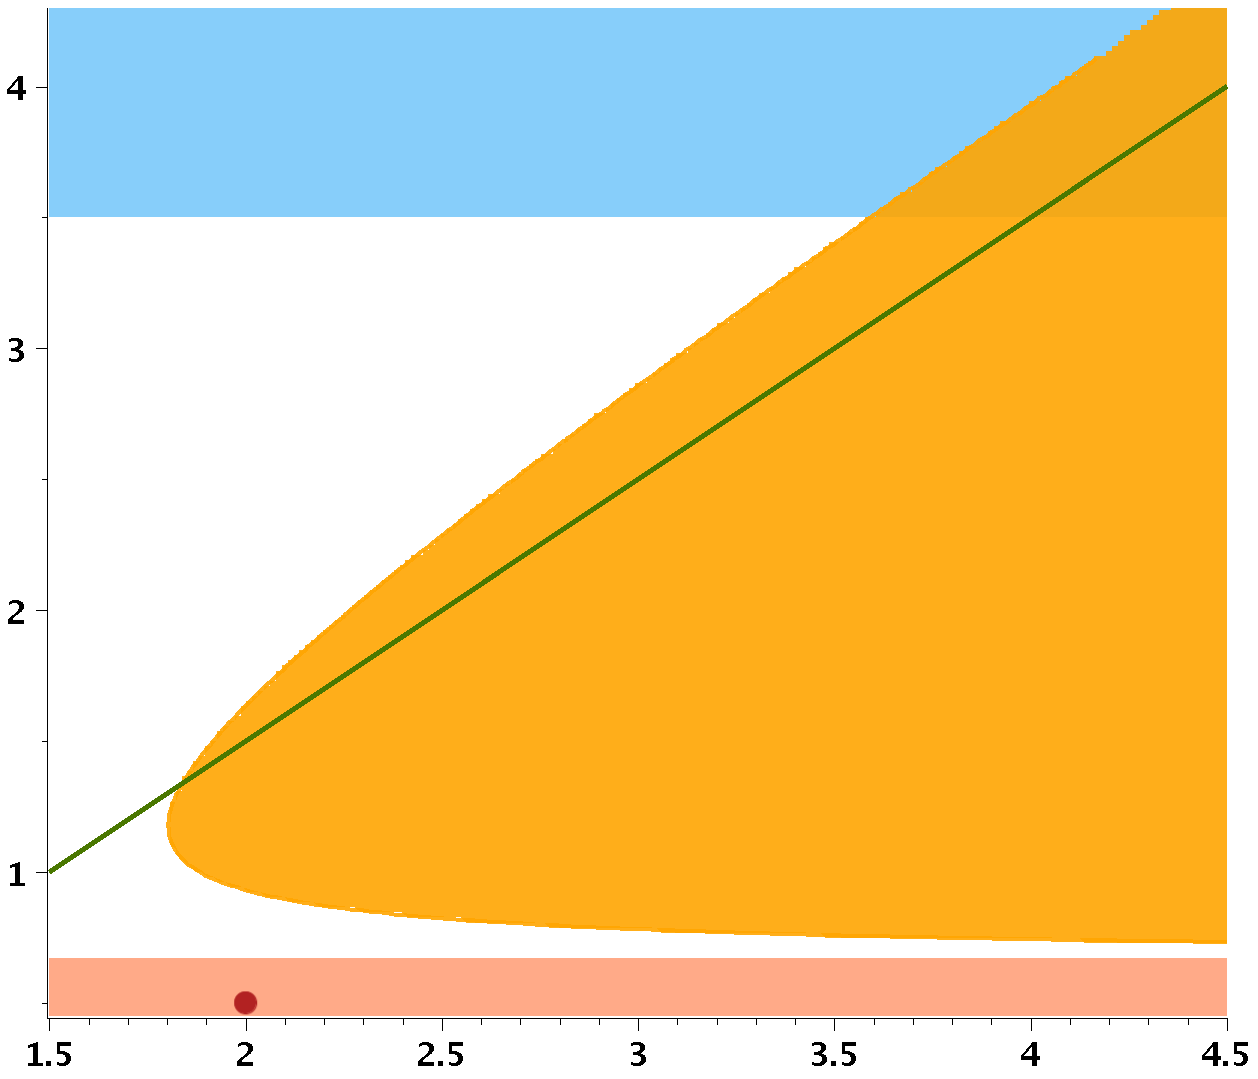
\includegraphics[width=0.59\textwidth]{Plots/Plots_SingleExp_ExpSamples.png}};
				    \begin{scope}[x={(image.south east)},y={(image.north west)}]
				    	
				    	% Help lines: Comment out once finished % 
				   		%\draw[help lines,xstep=.1,ystep=.1] (0,0) grid (1,1);
				    	%\foreach \x in {0,1,...,9} { \node [anchor=north] at (\x/10,0) {0.\x}; }
				    	%\foreach \y in {0,1,...,9} { \node [anchor=east] at (0,\y/10) {0.\y}; }
				    	
				    	%\node[draw=none] at (0.45, 0.15) {\tiny $\BKW2 \leq \ENUM2 \leq \BKW \leq \ENUM$};
				    	%\node[draw=none, color=black] at (0.6, 0.52) {Quantum reduction};
				    
				    	\draw[fill=LightSkyBlue, opacity=0.9] (1.0, 0.6) rectangle (1.05, 0.65) node[yshift=-2ex, xshift=17ex]{$\DUALH \leq \BKW2 \leq \DUALOne \leq \BKW$};
				    	\draw[fill=Orange] (1.0, 0.5) rectangle (1.05, 0.55) node[yshift=-2ex, xshift=17ex] { $\DUALH \leq \BKW2 \leq \BKW \leq \DUALOne$}; 
				    	\draw[fill=LightSalmon, opacity=0.8] (1.0, 0.4) rectangle (1.05, 0.45) node[yshift=-2ex, xshift=17ex] {$\BKW2 \leq \BKW \leq \DUALH \leq \DUALOne $};
				    	\draw[fill=white] (1.0, 0.3) rectangle (1.05, 0.35) node[yshift=-2ex, xshift=17ex] {$\BKW2 \leq \DUALH \leq \BKW \leq \DUALOne$};
				    	
				    	\node[draw=none, xshift=16ex, yshift=1.5ex] at (0.03, 0.17) {\scriptsize $\BKW2 = 0.92$};
				    	\node[draw=none, xshift=15ex, yshift=1.5ex] at (0.04, 0.13) {\scriptsize $\BKW = 1.16$};
				    	\node[draw=none, xshift=18ex, yshift=1.8ex] at (0.015, 0.09) {\scriptsize $\DUALH = 1.0$};
				    	\node[draw=none, xshift=16ex, yshift=1.9ex] at (0.03, 0.05) {\scriptsize $\DUALOne = 4.0$};
				    	
				    	\node[draw=none, rotate=35] at (0.37, 0.42){$\alpha q > \sqrt{n}$};
				    	
				    	\node[draw=none] at (0.5, -0.03) {$\cq$};
				    	\node[draw=none] at (-0.02, 0.5) {$\ca$};
				    	
				    \end{scope}
		\end{tikzpicture}
		\caption{
				 Same as above but for \emph{exponential} number of \LWE samples.
		}
		\label{fig:SingExpExpSamples}
		\end{subfigure}
		\caption[Comparison of algorithms for \LWE with polynomial and exponential number of samples]{Asymptotical behaviour of various algorithms for \LWE: lattice-based Enumeration or Dual attacks vs.\ combinatorial \BKW.}
		\label{fig:LWEPlots}
\end{figure}
